\documentclass{article}
\usepackage{listings}
\usepackage{geometry}
\usepackage{amsmath,amsthm,amssymb}
\usepackage{hyperref}
\usepackage{color}
\usepackage{mathtools}
\usepackage[dvipsnames]{xcolor}
\usepackage{tikz-cd}

% mathbb shortcuts
\newcommand{\Z}{\mathbb{Z}}
\newcommand{\N}{\mathbb{N}}
\newcommand{\Q}{\mathbb{Q}}
\newcommand{\R}{\mathbb{R}}
\newcommand{\C}{\mathbb{C}}
\newcommand{\F}{\mathbb{F}}
\newcommand{\T}{\mathbb{T}}
\newcommand{\HH}{\mathbb{H}}
\newcommand{\RP}{\mathbb{RP}}
\newcommand{\PP}{\mathbb{P}}
\newcommand{\A}{\mathbb{A}}
\newcommand{\E}{\mathbb{E}}

% mathfrak shortcuts
\newcommand{\fI}{\mathfrak{I}}
\newcommand{\fA}{\mathfrak{A}}
\newcommand{\fG}{\mathfrak{G}}

% mathcal shortcuts
\newcommand{\cA}{\mathcal{A}}
\newcommand{\cU}{\mathcal{U}}
\newcommand{\cR}{\mathcal{R}}
\newcommand{\cP}{\mathcal{P}}
\newcommand{\cB}{\mathcal{B}}
\newcommand{\cC}{\mathcal{C}}
\newcommand{\cF}{\mathcal{F}}
\newcommand{\cS}{\mathcal{S}}

\newcommand{\Aut}{\textrm{Aut}}
\newcommand{\degg}{\textrm{deg}}
\newcommand{\Hom}{\textrm{Hom}}
\newcommand{\conj}{\textrm{conj}}
\newcommand{\Gal}{\textrm{Gal}}
\newcommand{\disc}{\textrm{disc}}
\newcommand{\supp}{\textrm{supp}}
\newcommand{\Jac}{\textrm{Jac}}
\newcommand{\Der}{\textrm{Der}}
\newcommand{\Spec}{\textsf{Spec}\,}
\newcommand{\im}{\textrm{im}\,}

% mathsf shortcuts
\newcommand{\Cell}{\textsf{Cell}}

\newcommand{\clr}{\color{red}}

\newtheorem{lemma}{Lemma}
\newtheorem{definition}{Definition}
\theoremstyle{definition}




\begin{document}

\begin{center}
	\large \textbf{GRST Notes: Research Ideas (January 25, 2017)} \\
\end{center}

This week, Sam talked about some ideas he had about possible directions for research. In this post, all sheaves have values in $\textsf{Vect}$. 

\section{Random Sheaves}
An interesting concept to consider is the notion of a random sheaf, and how to properly define one. We will discuss two dual methods for obtaining such a sheaf: a top-down method in which we begin at the highest dimensional cell, and work our way down in dimension; and a bottom-up method in which we start with 0- and 1- cells, and work our way up in dimension. 

\subsection{Top-Down Approach}

We begin with Sam's algorithm to construct a random sheaf from the top-down. The aim is to define a sheaf on a fixed $n$-dimensional cell complex $X$ where the stalk (a vector space) over each cell is predetermined. We call such an object a \textbf{Liorian}. To demonstrate the algorithm, we will consider the following cell complex as an example. 	

\begin{figure}[!htbp]
\centering
	\includegraphics[width=0.3\textwidth]{images/triangle_step1.eps}
\end{figure}

We begin by defining maps out of the $(n-1)$-cells. Note that there are no maps out of the $n$-cells, since they are of the highest dimension. In the case of our example, we will be defining maps out of the $1$-cells, denoted by the arrows in red. The maps are defined one cell at a time, so suppose we focus on the map out of the cell $z$.  But first, we need some terminology.

\begin{definition}
Suppose $(P, \leq)$ is a pre-order. The \textbf{open star} of a point $x \in P$ is defined to be the set $U_x = \{y \in P \, | \, x \leq y\}$.
\end{definition}

The open star is simply the set of higher-dimensional cells of which the cell $x$ is a face. Viewing the cell complex $X$ as a poset, we take the open star of the cell $z$, along with all maps connecting these points. In this first step, the result is a simple diagram.

\[
\begin{tikzcd}
	T \\
	z \arrow{u}
\end{tikzcd}
\]

Next, we remove $z$ along with all maps out of $z$ from the open star and we denote this the \textbf{reduced open star}. We then take the limit of the reduced open star. The reduced open star in this case is just a single point, so the limit $L_z$  will simply be the stalk over $T$, along with the identity map into $T$. The map from $z$ into $T$, denoted $\phi_{z,T}$ can be defined by choosing a random map, $\alpha_z$ from $z$ into $L_z$, as shown in the following diagram. 

\[
\begin{tikzcd}
	T \\
	L_z \arrow{u}{\textrm{Id}}\\
	z \arrow{u}{\alpha_z} \arrow[bend right=50,swap,red]{uu}{\phi_{z,T}}
\end{tikzcd}
\]

Here, $\phi_{z,T} = \alpha_z$, so defining the map from $z$ into $T$ reduces to choosing a random map from the stalk of $z$ into the stalk of $T$. The same procedure can be done for maps out of $x$ and $y$. The reason for taking limits may not be clear in this initial step of the algorithm, but this will be essential in the later steps.\\

\begin{figure}[!htbp]
\centering
	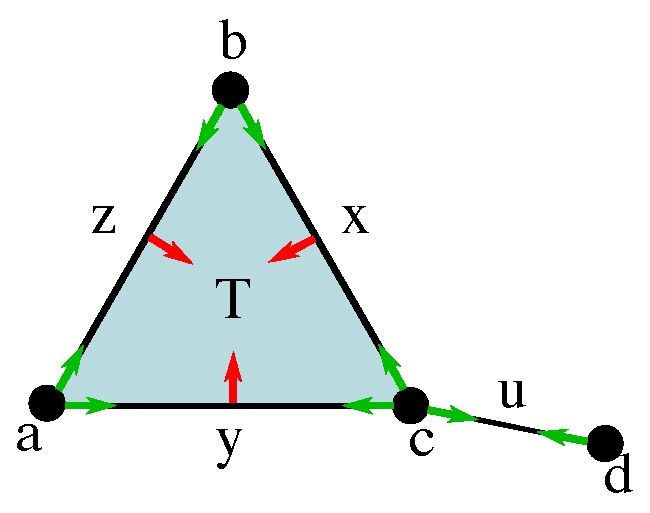
\includegraphics[width=0.3\textwidth]{images/triangle_step2.eps}
\end{figure}

Now that all maps out of $(n-1)$-cells are determined, we move on to maps out of $(n-2)$-cells. In our example, these are the maps out of the $0$-cells, which are shown in green. Let's start by considering the maps out of the cell $a$. Once again, we start off by taking the open star of $a$:

\[
\begin{tikzcd}
	& T & \\
	z \arrow[red]{ur} &  & y \arrow[red]{ul} \\
	& a \arrow[ForestGreen]{ul} \arrow[ForestGreen]{ur} & 
\end{tikzcd}
\]

Next, we remove $a$ and all maps out of $a$ to get the reduced open star and take the limit of the diagram. This gives us the limit $L_a$, and two maps $p_1 : L_a \rightarrow z$ and $p_2: L_a \rightarrow y$. We choose a random map $\alpha_a: a \rightarrow L_a$, and the green arrows are then defined by composition. Explicitly, we have $\phi_{a,z} = p_1 \circ \alpha_a$ and $\phi_{a,y} = p_2 \circ \alpha_a$.  This scenario can be seen in the following diagram. 

\[
\begin{tikzcd}
	& T & \\
	z \arrow[red]{ur} &  & y \arrow[red]{ul} \\
	& L_a \arrow[swap,"p_1"]{ul} \arrow["p_2"]{ur} & \\
	& a \arrow{u}{\alpha_a} \arrow[ForestGreen,bend left]{uul}{\phi_{a,z}} \arrow[swap, ForestGreen, bend right,"\phi_{a,y}"]{uur} &
\end{tikzcd}	
\]

By choosing a random map into the limit, and defining the $\phi$ maps by composition,  we ensure that commutativity of the diagram holds. We then repeat this procedure for all other $0$ cells, to obtain a consistent set of maps. Note that since $u$ is not the face of any other cell, defining maps into $u$ will be similar to how we defined maps into $T$. Namely, they will simply be a random choice of a map from the stalk of $c$ or $d$ into the stalk of $u$. \\

This was a fairly simple example to complete, but the algorithm is similar for cell complexes with higher dimensional cells. We simply continue to iterate the procedure dimension-by-dimension until we reach the $0$-cells, at which point we will have fully defined the sheaf. \\

\subsection{Bottom-Up Approach}
\begin{figure}[!htbp]
\centering
	\includegraphics[width=0.3\textwidth]{images/triangle_step3.eps}
\end{figure}

Next, we discuss the dual bottom-up approach to building a random sheaf. The main difference will be the use of a colimit rather than a limit, and building up the maps into each cell dimension by dimension. Once again, we start with a Liorian: a cell complex $X$ where stalks over each cell are predetermined. We will use the same Liorian to demonstrate the procedure, and we start by defining maps into $1$-cells, which are shown in green above. We begin by focusing on maps into $z$.

\begin{definition}
Suppose $(P, \leq)$ is a pre-order. The \textbf{closure} of a point $x \in P$ is defined to be the set $V_x = \{y \in P \, | \, y \leq x\}$.
\end{definition}

Here, we are simply taking all lower dimensional cells that are faces of the given cell $z$. We take the closure of the cell $z$, along with all maps between the points in the closure. Similar to the reduced open star, we remove $z$ along with all maps into $z$ and denote this the \textbf{reduced closure} of $z$. We take the colimit of the resulting diagram, to obtain the colimit $L_z$ along with maps $q_1: a  \rightarrow L_z$ and $q_2: b\rightarrow L_z$. We choose a random map $\alpha_z: L_z \rightarrow z$ and define the maps into $z$, $\phi_{a,z}$ and $\phi_{b,z}$ to be the composition as shown in the diagram below.

\[
\begin{tikzcd}
	& z & \\
	& L_z \arrow{u}{\alpha_z} & \\
	a \arrow[swap]{ur}{q_1} \arrow[bend left, ForestGreen]{uur}{\phi_{a,z}} & & b \arrow{ul}{q_2} \arrow[swap, bend right, ForestGreen]{uul}{\phi_{b,z}}
\end{tikzcd}
\]

It is clear that we can do this for all $1$-cells, and then continue with higher dimensional cells until all maps are defined. \\

\subsection{Extending Sheaves on Graphs}
During the discussion about building random sheaves, Jakob suggested a way to modify the algorithm to extend a sheaf on a graph to a sheaf on its clique complex. Here, we begin with a sheaf on a graph $X_1$. This implies the stalks over all cells in the graph are chosen, and a consistent set of maps from $0$ cells into $1$ cells is also chosen. For this post, we will continue to use the following example, noting the $2$-cell is not present.\\

\begin{figure}[!htbp]
\centering
	\includegraphics[width=0.3\textwidth]{images/graph.eps}
\end{figure}

Now, we consider the clique complex $X$ of the graph and we denote its $n$-skeleton by $X_n$. We will iteratively define the stalks and maps in the higher dimensional cells beginning with $X_2$. The $2$-skeleton of the clique complex of the above graph is shown in the following figure.

\begin{figure}[!htbp]
\centering
	\includegraphics[width=0.3\textwidth]{images/graph2.eps}
\end{figure}

During this step, we must define the stalks on all $2$ cells and also all maps into $2$-cells. In our example, we must define the stalks over $T$ and define the maps represented by the red arrows. This is done by following the procedure in the bottom-up approach. We define the stalk over $T$ to be the colimit of its reduced closure (denoted by $L_T$), and define the maps into $T$ (the red maps) to be the maps into the colimit.

\[
\begin{tikzcd}
	& L_T & \\
	x \arrow[red]{ur}{\phi_{x,T}} & y \arrow[swap, red]{u}{\phi_{y,T}} & z \arrow[swap,red]{ul}{\phi_{z,T}} \\
	a \arrow{ur} \arrow{urr} & b \arrow{ur} \arrow{ul} & c \arrow{ul} \arrow{ull}
\end{tikzcd}	
\]

In the case of this example, we are done. However, if there were more $2$-cells, we would simply repeat this procedure until we have a sheaf on $X_2$. Then, we continue this process for higher dimensional cells until we have a sheaf on $X$. \\

Note that using this extension method, the sheaf on the graph was the only data we needed to predetermine. All other stalks and maps are well-defined using this colimit procedure. Thus, each sheaf on a graph will result in a unique sheaf on its clique complex with this algorithm. In contrast, when we define sheaves on a Liorian, we needed to choose a random map into each limit/colimit when defining maps into or out of cells. With this formulation, we can think about the space of all possible maps, and which collections of maps will ultimately result in a sheaf. We discuss this further in the next section.\\

One interesting aspect of the graph extension approach is that we can build a random sheaf by defining a random graph. In other words, the randomness comes from a random cell complex rather than a choice of random maps. It would be interesting to study asymptotic properties of random sheaves built in this manner, since this is similar to how random graph theory was extended to random clique complexes in the work of Kahle ({\clr cite something}). 


\section{Moduli Spaces of Sheaves}
As we hinted in the previous section, it would be interesting to understand all possible sheaves given a Liorian. There are two different viewpoints that we can take with this: an iterative viewpoint mimicing the iterative process to build the random sheaf, and a consolidated viewpoint which looks at entire procedure all at once. In this section, we will use the top-down approach, but the discussion can be reworded in the context of the bottom-up approach.

\subsection{Iterative Viewpoint}
\begin{figure}[!htbp]
\centering
	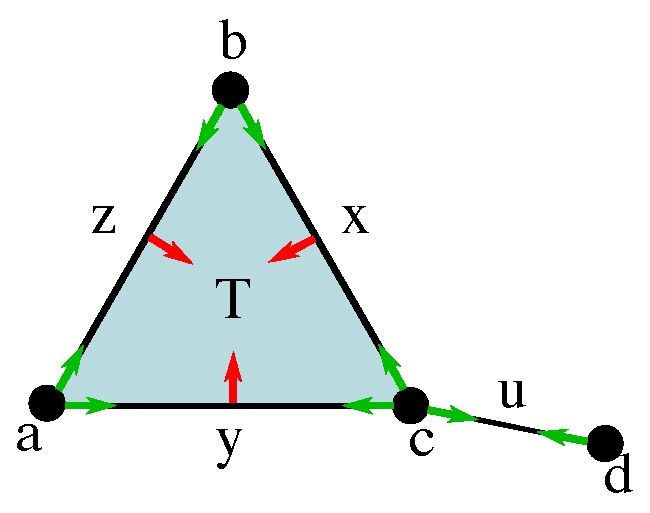
\includegraphics[width=0.3\textwidth]{images/triangle_step2.eps}
\end{figure}

Consider the construction of the sheaf in the top-down approach, and we continue with the same cell complex as an example. For concreteness, suppose that the vector spaces over the cells $z$ and $T$ are $z =k^p$ and $T = k^q$, where $k$ is a field. Any map $\phi_{z,T} : k^p \rightarrow k^q$ can be represented as a matrix $(x_{i,j})_{1\leq i \leq p, 1 \leq j \leq q}$ of $pq$ variables, so we can think of any such matrix as being a point in $k^{pq}$. We obtain one matrix for each map we aim to define. The space of all matrices for maps coming out of $1$-cells is $k^{N_1}$, where $N_1$ is the sum of the number of variables for each of these matrices.\\

Note that at this first step, there are no restrictions on these maps, since no other maps have been defined yet and thus there are no commutativity relations to enforce. Once we choose a set of maps out of $1$-cells (a point in $k^{N_1}$), we can move to lower dimensions. We can consider the space of all matrices for maps coming out of $0$-cells, which we denote $k^{N_0}$, (where $N_0$ is the sum of the number of variables for all matrices out of $0$-cells), but not every point in this space will result in a set of matrices that satisfy all commutativity relations. In fact, enforcing the commutativity of the diagrams will give us a collection of polynomial equations where the variables are elements of these matrices; we denote this collection of equations $\cP_0$. Therefore, a consistent set of matrices that satisfies all the sheaf conditions is a point in $k^{N_0}$ that satisfies all polynomial equations in $\cP_0$. In other words, it is a point on the variety $S_0 = V(\cP_0)$ in $k^{N_0}$.\\

It turns out that all polynomials in $\cP_0$ are linear equations. Consider the maps $\phi_{a,y}$ and $\phi_{a,z}$ out of the $0$-cell $a$. The commutativity relation this must satisfy is: $\phi_{z,T} \circ \phi_{a,z} - \phi_{y,T} \circ \phi_{a,y}  = 0$. Note that $\phi_{z,T}$ and $\phi_{y,T}$ are already well defined (since they are maps out of a higher dimensional cell), whereas $\phi_{a,z}$ and $\phi_{a,y}$ are to be determined, so they are matrices of variables. Additionally, since these are all matrices, composition is simply matrix multiplication. Thus, we obtain one linear equation for each component of the matrix.  \\

In the case of the cell complex above, $S_0$ defines the space of all possible sheaves, since the construction is complete after defining maps out of the $0$-cells. However, suppose that the maximum dimension in the cell complex is $n$. There are no commutativity relations for maps out of $(n-1)$-cells, so we are free to choose any point in $k^{N_{n-1}}$. The next step is to define the maps out of $(n-2)$-cells. By the argument above, the space of all possible maps out of $(n-2)$ cell is $k^{N_{n-2}}$, where $N_{n-2}$ is the number of variables for each of these matrices. We will get a collection of polynomials, $\cP_{n-2}$, that these variables must satisfy, and the resulting variety is $S_{n-2} = V(\cP_{n-2})$. After choosing a point in this variety, we continue this procedure until we reach the variety $\cS_0$. Then, any point in $S_0$ will result in a sheaf. However, an important point to note is that each variety $S_i$ is dependent on the choice of point in the previous variety $S_{i+1}$. A visual representation of this idea is in the following figure. 

\begin{figure}[!htbp]
\centering
	\includegraphics[width=0.3\textwidth]{images/variety2_fixed.eps}
\end{figure}


It would be interesting to study these sheaves, and furthermore investigate the moduli spaces of these sheaves. The moduli space is obtained by identifying equivalent sheaves. Recall that sheaves are functors from the category $\textsf{Cell}(X)$ into the category $\textsf{Vect}$. Thus, two sheaves $F$ and $G$ are equivalent if and only if there exists a natural isomorphism $\alpha$ between $F$ and $G$. Recasting this in terms of the construction presented in this post, two sheaves $F$ and $G$ over a fixed Liorian $X$ are equivalent if there exist changes of bases for the vector spaces over each cell such that all maps are equal.\\

Explicitly, consider two sheaves over our example Liorian, where we denote the maps $\phi_{i,j}$ and $\psi_{i,j}$. Two sheaves are equivalent if there exists a set of invertible matrices $\{M_k\}$ (one map for each cell) such that
\begin{equation}
	\psi_{i,j} = M_i \circ \phi_{i,j}\circ M^{-1}_j.
\end{equation}
We note that changing bases still preserves all commutativity relations. For example, consider the two maps from $a$ into $T$. When we look at the maps with a change of basis, we get
\begin{equation}
	(M_a \phi_{a,z} M^{-1}_z) \circ (M_z \phi_{z,T} M^{-1}_T) = M_a \phi_{a,z} \phi_{z,T} M_T^{-1}
\end{equation}
\begin{equation}	
	(M_a \phi_{a,y} M^{-1}_y) \circ (M_y \phi_{y,T} M_T^{-1}) = M_a \phi_{a,y} \phi_{yT} M_T^{-1}
\end{equation}
which is equal since $\phi_{a,z} \phi_{z,T} = \phi_{a,y} \phi_{yT}$.

\subsection{Consolidated Approach and Approximate Sheaves}
Finally, we will consider the consolidated approach. Instead of looking at this procedure iteratively, we can look at all of the matrices for all of the unknown maps at once. The set of all such matrices would be in $k^N$ (where $N$ is the number of variables required to define all maps), and we would get a large collection of polynomials $\cP$, which would form a variety $S = V(\cP)$. Here the polynomials will not be linear, but they will be quadratic instead. This is because every commutativity relation will be in the form of an equation such as $\phi_{z,T} \circ \phi_{a,z} - \phi_{y,T} \circ \phi_{a,y}  = 0$. If each $\phi$ is a matrix of variables, then this matrix equation will give a set of quadratic equations for each element of the matrix. We can ask similar questions here about the variety and moduli space of sheaves and investigate their properties.\\

The final idea is that of an approximate sheaf. When we obtain sheaves in real life, it is highly unlikely that all of the maps will commute properly, but it may be ``close'' to being a sheaf. Is there a way to put a metric on the space $k^N$ and ask what is the closest sheaf to the approximate sheaf?

\begin{figure}[!htbp]
\centering
	\includegraphics[width=0.3\textwidth]{images/variety3.eps}
\end{figure}


\end{document}